\section{Method}
\subsection{Agent-Based Modeling Approach}
An Agent-based modeling (ABM) was selected as the methodological framework for this research due to its ability to capture the complex interactions and emergent behaviors that characterize circular economy systems \cite{Hansen2020}. In contrary to traditional system dynamics models, ABM allows for the representation of agents with diverse characteristics, decision-making processes, and adaptive behaviors, making it particularly suitable for investigating a socio-technical problem such as battery circularity.

The ABM approach enables us to model the four key stakeholder groups in the battery lifecycle:
\begin{enumerate}
    \item EV owners
    \item Car manufacturers
    \item Recycling facilities
    \item battery refurbishers
\end{enumerate}
Each agent class has distinct attributes, decision rules, and interactions that collectively determine the flow of batteries through the system. By implementing this model, we can explore how individual-level decisions and constraints aggregate to produce system-level outcomes, including recycling rates, second-life utilization, and material recovery.

\subsection{Model Design}
The model was implemented in Python using object-oriented programming principles. We developed a modular architecture with separate agent classes for each , for simplicity, and demarcation purposes we consider cars as a battery; thus, a battery class for tracking battery attributes and status changes, and a main model class that coordinates agent interactions and aggregates system-level metrics.

The model implements a Mesa-based architecture with the following key components:
\begin{itemize}
    \item A base \texttt{Agent} class that extends Mesa's agent implementation with location-based functionality
    \item Four specialized agent types: EV owners, car manufacturers, recycling facilities, and battery refurbishers
    \item A \texttt{Battery} class representing the physical batteries that flow through the system
    \item A state-transition mechanism for batteries modeled as the \texttt{BatteryStatus} enum
\end{itemize}

\subsubsection{Conceptual Model}
The conceptual framework of our agent-based model represents the circular EV battery system as a network of interacting agents with defined behaviors, decision rules, and state transitions. As illustrated in Appendix A (Figure \ref{fig:class_diagram}), our model implements a comprehensive object-oriented architecture with five primary classes that correspond directly to the key components in the battery lifecycle.

Our model's architecture is built on the Mesa framework, with a clear hierarchical structure:
\begin{itemize}
    \item A base \texttt{Agent} class extends Mesa's agent implementation, providing common functionality such as location tracking and movement
    \item The \texttt{Battery} class acts as a central entity that flows through the system with its own lifecycle state transitions modeled through the \texttt{BatteryStatus} enum (NEW → IN\_USE → END\_OF\_LIFE → COLLECTED → RECYCLED/REFURBISHED)
    \item Four specialized agent classes (\texttt{EVOwner}, \texttt{CarManufacturer}, \texttt{RecyclingFacility}, and \texttt{BatteryRefurbisher}) implement domain-specific behaviors and decision-making processes
\end{itemize}

The conceptual model captures three key circular pathways that are directly implemented in our codebase:
\begin{enumerate}
  \item \textbf{Production-Use-Collection cycle}: Implemented through the interaction between \texttt{EVOwner.make\_purchase\_decision()} and \texttt{CarManufacturer.produce\_battery()} methods, with end-of-life handling managed via \texttt{EVOwner.handle\_battery\_replacement()}.
  
  \item \textbf{Second-life pathway}: Operationalized through \texttt{Battery.is\_suitable\_for\_second\_life()} checks and the \texttt{BatteryRefurbisher.refurbish\_battery()} method, which determines success based on technical capability and battery health.
  
  \item \textbf{Recycling pathway}: Implemented in the \texttt{RecyclingFacility.process\_battery()} method, which handles material recovery with realistic processing timeframes and efficiency factors.
\end{enumerate}

Our implementation includes sophisticated agent behaviors that reflect real-world decision processes. For example, \texttt{EVOwner} agents have heterogeneous attributes (income, environmental consciousness) that influence their end-of-life decisions, with more environmentally conscious owners more likely to choose refurbishment pathways as implemented in the \texttt{make\_end\_of\_life\_decision()} method.

The model also incorporates realistic constraints such as processing capacity limitations (\texttt{processing\_capacity} attributes in facility agents), operational dynamics including facility downtime (\texttt{operational} and \texttt{downtime\_counter} attributes), and waiting periods before battery handoffs (\texttt{eol\_waiting\_time} in \texttt{EVOwner}).

\subsubsection{Formal Model}
The formal model defines the mathematical representations and algorithms used to implement the conceptual framework. Key formal elements include:

\begin{itemize}
  \item \textbf{Agent state variables}: Each agent type maintains internal state variables that evolve over time. For example, batteries are modeled with a health parameter $h$ ($0 \leq h \leq 1$) that degrades according to a non-linear function:
  
  \begin{equation}
  h_t = h_{t-1} - \alpha_p \times d_r \times c
  \end{equation}
  
  where $h_t$ is the health at time $t$, $d_r$ is the base degradation rate, $c$ is the number of cycles, and $\alpha_p$ is a phase-dependent factor that equals 0.7 for the initial phase (cycle count < 200), 1.0 for the middle phase (200 < cycle count < 1000), and 1.5 for the end-of-life phase (cycle count > 1000).
  
  \item \textbf{Decision rules}: Formalized as probability functions. For example, the probability of an EV owner purchasing a new battery is modeled as:
  
  \begin{equation}
  P(\text{purchase}) = \begin{cases} 
  0.8 & \text{if no battery} \\
  0.8 & \text{if battery health } < \theta_{EOL} \\
  0.01 + 0.05 \times (\frac{I}{100000}) + 0.02 \times E_c + \min(0.7, \frac{A}{120}) & \text{otherwise}
  \end{cases}
  \end{equation}
  
  where $\theta_{EOL}$ is the end-of-life threshold, $I$ is owner income, $E_c$ is environmental consciousness, and $A$ is the battery age in months.
  
  \item \textbf{Facility processing dynamics}: Modeled as queuing systems with processing capacity constraints and efficiency parameters. For example, material recovery at recycling facilities is calculated as:
  
  \begin{equation}
  M_{recovered} = \sum_{b \in \text{batteries}} \sum_{m \in \text{materials}} Q_m \times \eta \times (0.8 + 0.2 \times h_b)
  \end{equation}
  
  where $Q_m$ is the quantity of material $m$ in a battery, $\eta$ is the facility efficiency rate, and $h_b$ is the health of battery $b$.
\end{itemize}

The model uses a discrete time-step approach with each step representing one month. The scheduling mechanism processes agent actions in the following order each month: battery degradation, owner decisions, manufacturer operations, facility processing, and metric calculation.

\subsubsection{Battery Agents}
The battery class is a central component of the model, representing individual EV batteries with the following key attributes:

\begin{itemize}
  \item Health status (0-1 scale): Batteries above 0.8 are considered in good condition, those between 0.6-0.8 are suitable for second-life applications, and those below 0.6 require recycling.
  \item Age (in months): Tracking the time since manufacturing.
  \item Current capacity (kWh): Representing the usable energy storage.
  \item Status: Tracking the battery's position in the lifecycle (new, in-use, end-of-life, collected, refurbished, or recycled).
  \item Cycle count: Number of charge-discharge cycles completed.
\end{itemize}

We implemented a realistic non-linear degradation model that captures the typical three-phase degradation pattern observed in lithium-ion batteries: an initial slow degradation phase, a mid-life linear degradation phase, and an accelerated end-of-life degradation phase \cite{YOU2024}.

\subsubsection{Owner Agents}
EV owner agents represent vehicle users with varying levels of:

\begin{itemize}
  \item Income: Influencing purchase decisions and replacement frequency.
  \item Environmental consciousness: Affecting end-of-life decisions regarding recycling versus refurbishment.
  \item Ownership duration: Tracking how long they've owned their current battery.
\end{itemize}

Owner agents make two critical decisions that impact battery circularity:

\begin{itemize}
  \item Purchase decisions: Based on current battery condition, age, and owner attributes.
  \item End-of-life handling decisions: Choosing between recycling, refurbishment, or continued use based on battery health and the owner's environmental consciousness.
\end{itemize}

\subsubsection{Manufacturer Agents}
Car manufacturer agents produce new batteries and manage the take-back of end-of-life batteries. Their key attributes include:

\begin{itemize}
  \item Production capacity: Number of batteries they can produce per time step.
  \item Recycling commitment: Probability of accepting end-of-life batteries (representing extended producer responsibility).
  \item Warranty policies: Age and health thresholds for warranty coverage.
\end{itemize}

Manufacturers decide whether to direct collected batteries to recycling or refurbishment based on the battery's condition, implementing the critical sorting function that determines a battery's second-life potential.

\subsubsection{Recycling Facility Agents}
Recycling facility agents process end-of-life batteries to recover valuable materials. Their key attributes include:

\begin{itemize}
  \item Processing capacity: Number of batteries they can handle per time step.
  \item Efficiency rate: Percentage of materials successfully recovered during recycling.
  \item Processing time: Realistic time delays for battery processing.
  \item Operational status: Accounting for potential facility downtime.
\end{itemize}

\subsubsection{Battery Refurbisher Agents}
Battery refurbisher agents convert suitable end-of-life batteries for second-life applications, primarily grid energy storage. Their key attributes include:

\begin{itemize}
  \item Technical capability: Success rate in refurbishing batteries.
  \item Processing capacity: Number of batteries they can refurbish per time step.
  \item Assessment procedures: Evaluating battery suitability for second-life applications.
\end{itemize}

\subsection{Simulation Scenarios}
We designed five experimental scenarios to investigate the impact of various technical, economic, and policy parameters on battery circularity rates:

\begin{table}[ht]
\centering
\caption{Parameter values across simulation scenarios}
\label{tab:scenario_params}
\begin{tabular}{lccccc}
\toprule
\textbf{Parameter} & \textbf{Baseline} & \textbf{Enhanced} & \textbf{Policy-Driven} & \textbf{Lower} & \textbf{Combined} \\
 & & \textbf{Refurbishment} & \textbf{Recycling} & \textbf{Threshold} & \textbf{Approach} \\
\midrule
Technical capability & 0.7 & \textbf{0.9} & 0.7 & 0.7 & \textbf{0.9} \\
Refurbisher capacity & 2 & \textbf{8} & 3 & 2 & \textbf{8} \\
Recycling commitment & 0.75 & 0.75 & \textbf{0.95} & 0.75 & \textbf{0.95} \\
Second-life threshold & 0.6 & 0.6 & 0.6 & \textbf{0.4} & \textbf{0.4} \\
\bottomrule
\end{tabular}
\end{table}

Each scenario was run for 500 time steps (representing months) with 10 different random seeds to ensure statistical robustness. The model tracked key metrics including recycling rates, second-life conversion rates, material recovery, grid storage creation, and facility utilization.

\subsection{Validation and Verification}
To ensure the reliability and accuracy of our model, we conducted comprehensive validation and verification procedures:

\subsubsection{Face Validation}
We validated the conceptual model through interviews with domain experts from the Dutch waste management sector and battery research community at TU Delft. The agent structure, decision rules, and system dynamics were confirmed to align with real-world processes and stakeholder behaviors.

\subsubsection{Internal Verification}
Code verification was performed through:
\begin{itemize}
  \item Unit testing of agent classes and their behaviors
  \item Conservation checks to verify that no batteries "disappear" from the system
  \item Boundary testing with extreme parameter values
  \item Debugging output for tracking agent state transitions
\end{itemize}

\subsubsection{Parameter Verification}
Parameter values were derived from literature and validated against real-world data where available. Battery degradation patterns were calibrated using empirical data from EV battery aging studies \cite{Hu2017}. Facility processing capacities and efficiencies were based on industry benchmarks.

\subsubsection{Sensitivity Analysis}
We conducted sensitivity analysis on key parameters to assess model robustness and identify critical factors. Figure \ref{fig:sensitivity} shows the impact of varying four key parameters on recycling and second-life rates.

\begin{figure}[ht]
\centering
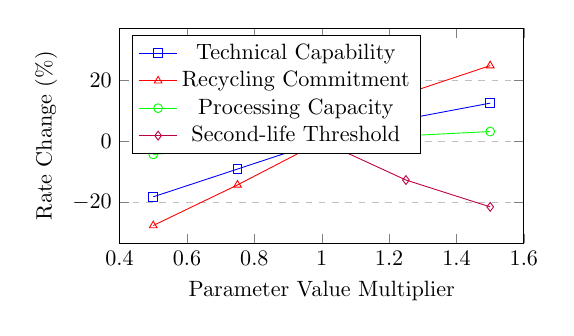
\begin{tikzpicture}[scale=0.8, transform shape]
\begin{axis}[
    width=8cm,
    height=5cm,
    xlabel={Parameter Value Multiplier},
    ylabel={Rate Change (\%)},
    legend pos=north west,
    ymajorgrids=true,
    grid style=dashed,
]

\addplot[
    color=blue,
    mark=square,
    ]
    coordinates {
    (0.5,-18.2)(0.75,-9.1)(1,0)(1.25,7.3)(1.5,12.5)
    };
    
\addplot[
    color=red,
    mark=triangle,
    ]
    coordinates {
    (0.5,-27.6)(0.75,-14.3)(1,0)(1.25,15.6)(1.5,24.8)
    };
    
\addplot[
    color=green,
    mark=o,
    ]
    coordinates {
    (0.5,-4.3)(0.75,-2.1)(1,0)(1.25,1.8)(1.5,3.2)
    };
    
\addplot[
    color=purple,
    mark=diamond,
    ]
    coordinates {
    (0.5,31.2)(0.75,14.9)(1,0)(1.25,-12.7)(1.5,-21.5)
    };
    
\legend{Technical Capability, Recycling Commitment, Processing Capacity, Second-life Threshold}
    
\end{axis}
\end{tikzpicture}
\caption{Sensitivity analysis showing the percentage change in second-life rates when varying key parameters}
\label{fig:sensitivity}
\end{figure}

The analysis revealed that technical capability and second-life threshold have the strongest influence on system performance, while processing capacity has a more modest impact. Interestingly, the second-life threshold exhibits a non-linear relationship, with disproportionately larger effects at lower values, suggesting a potential tipping point in the system.

\FloatBarrier
\section{Results}
Our agent-based model simulations reveal several key insights regarding battery circularity strategies in the Netherlands. The results demonstrate significant variations in performance across the experimental scenarios, with important implications for policy development and infrastructure planning.

\subsection{Battery Status Distribution}
The battery status distribution over time illustrates how batteries flow through different lifecycle stages across scenarios. Figure \ref{fig:battery_status} shows these distributions for the five scenarios.

\begin{figure}[htbp]
\centering
\begin{subfigure}{0.42\textwidth}
    \includegraphics[width=\textwidth]{figures/baseline_battery_status.png}
    \caption{Baseline scenario}
    \label{fig:battery_baseline}
\end{subfigure}
\hfill
\begin{subfigure}{0.42\textwidth}
    \includegraphics[width=\textwidth]{figures/enhanced_refurbishment_battery_status.png}
    \caption{Enhanced Refurbishment scenario}
    \label{fig:battery_enhanced}
\end{subfigure}

\vspace{0.2cm}
\begin{subfigure}{0.42\textwidth}
    \includegraphics[width=\textwidth]{figures/policy-driven_recycling_battery_status.png}
    \caption{Policy-Driven Recycling scenario}
    \label{fig:battery_policy}
\end{subfigure}
\hfill
\begin{subfigure}{0.42\textwidth}
    \includegraphics[width=\textwidth]{figures/lower_second-life_threshold_battery_status.png}
    \caption{Lower Second-Life Threshold scenario}
    \label{fig:battery_lower}
\end{subfigure}

\vspace{0.2cm}
\begin{subfigure}{0.42\textwidth}
    \includegraphics[width=\textwidth]{figures/combined_approach_battery_status.png}
    \caption{Combined Approach scenario}
    \label{fig:battery_combined}
\end{subfigure}
\caption{Battery status distribution over time across all scenarios}
\label{fig:battery_status}
\end{figure}

The baseline scenario (Figure~\ref{fig:battery_baseline}) shows a gradual buildup of recycled and refurbished batteries, with recycling becoming the dominant pathway by the end of the simulation period. In contrast, the enhanced refurbishment scenario (Figure~\ref{fig:battery_enhanced}) demonstrates a much higher proportion of refurbished batteries, indicating that improvements in refurbishment capabilities can substantially increase second-life utilization.

The policy-driven recycling scenario (Figure~\ref{fig:battery_policy}) results in the highest overall proper end-of-life management (combined recycling and refurbishment), demonstrating the effectiveness of strong producer responsibility policies. The lower second-life threshold scenario (Figure~\ref{fig:battery_lower}) achieves the most balanced distribution between recycling and refurbishment, suggesting that adjusting technical criteria for second-life eligibility can effectively maximize battery utilization before final recycling.

\subsection{Facility Processing}
Facility processing metrics provide insights into the operational aspects of the circularity system. Figure \ref{fig:facility_processing} shows the cumulative number of batteries processed through recycling and refurbishment pathways over time.

\begin{figure}[htbp]
\centering
\begin{subfigure}{0.42\textwidth}
    \includegraphics[width=\textwidth]{figures/baseline_facility_processing.png}
    \caption{Baseline scenario}
    \label{fig:facility_baseline}
\end{subfigure}
\hfill
\begin{subfigure}{0.42\textwidth}
    \includegraphics[width=\textwidth]{figures/enhanced_refurbishment_facility_processing.png}
    \caption{Enhanced Refurbishment scenario}
    \label{fig:facility_enhanced}
\end{subfigure}

\vspace{0.2cm}
\begin{subfigure}{0.42\textwidth}
    \includegraphics[width=\textwidth]{figures/policy-driven_recycling_facility_processing.png}
    \caption{Policy-Driven Recycling scenario}
    \label{fig:facility_policy}
\end{subfigure}
\hfill
\begin{subfigure}{0.42\textwidth}
    \includegraphics[width=\textwidth]{figures/lower_second-life_threshold_facility_processing.png}
    \caption{Lower Second-Life Threshold scenario}
    \label{fig:facility_lower}
\end{subfigure}

\vspace{0.2cm}
\begin{subfigure}{0.42\textwidth}
    \includegraphics[width=\textwidth]{figures/combined_approach_facility_processing.png}
    \caption{Combined Approach scenario}
    \label{fig:facility_combined}
\end{subfigure}
\caption{Cumulative facility processing across all scenarios}
\label{fig:facility_processing}
\end{figure}

The facility processing metrics reveal several key patterns. In the baseline scenario (Figure~\ref{fig:facility_baseline}), recycling dominates as the primary processing pathway. The enhanced refurbishment scenario (Figure~\ref{fig:facility_enhanced}) shows a significant increase in refurbishment rates, with the curves crossing around month 300, indicating that refurbishment eventually becomes the dominant pathway.

The policy-driven recycling scenario (Figure~\ref{fig:facility_policy}) demonstrates the strongest growth in recycling processing, as expected, while the lower threshold scenario (Figure~\ref{fig:facility_lower}) achieves the most balanced processing distribution. The combined approach (Figure~\ref{fig:facility_combined}) shows both high recycling and refurbishment rates, confirming the synergistic effect of implementing multiple policy and technical improvements simultaneously.

\subsection{Circularity Rates}
Figure \ref{fig:circularity_rates} presents the recycling and second-life rates across all scenarios, showing the percentage of total end-of-life batteries that are successfully recycled or refurbished.

\begin{figure}[htbp]
\centering
\includegraphics[width=0.75\textwidth]{figures/comparison_circularity_rates.png}
\caption{Circularity rates comparison across scenarios}
\label{fig:circularity_rates}
\end{figure}

The combined approach achieved the highest total circularity rate at 84\%, followed by the policy-driven scenario at 78\%, enhanced refurbishment at 78\%, lower threshold at 66\%, and baseline at 72\%. Notably, the lower threshold scenario achieved the lowest overall circularity rate but maintained a relatively high second-life rate at 24\%, suggesting that there may be a trade-off between optimizing for immediate circularity versus maximizing utility through extended use.

\subsection{Material Recovery}
The material recovery results shown in Figure \ref{fig:material_recovery} visualize how different materials (lithium, cobalt, nickel, and copper) are recovered across scenarios over time.

\begin{figure}[htbp]
\centering
\includegraphics[width=0.75\textwidth]{figures/comparison_material_recovery.png}
\caption{Material recovery over time for all scenarios}
\label{fig:material_recovery}
\end{figure}

Material recovery shows interesting temporal patterns. All scenarios exhibit an exponential growth pattern in recovery, with minimal differences in the first 60 months and increasingly divergent trajectories thereafter. The policy-driven recycling scenario achieved the highest cumulative recovery of critical materials, as expected given its focus on effective end-of-life management.

Interestingly, while the lower threshold scenario initially shows slower material recovery due to diverting more batteries to second life, it eventually catches up to a considerable extent, demonstrating that increased second-life utilization does not necessarily compromise long-term material recovery objectives. This supports the argument for a sequential circular economy approach that maximizes utility before recovery.